%%%%%%%%%%%%%%%%%%%%%%%%%%%%%%%%%%%%%%%%%
% Journal Article
% LaTeX Template
% Version 1.3 (9/9/13)
%
% This template has been downloaded from:
% http://www.LaTeXTemplates.com
%
% Original author:
% Frits Wenneker (http://www.howtotex.com)
%
% License:
% CC BY-NC-SA 3.0 (http://creativecommons.org/licenses/by-nc-sa/3.0/)
%
%%%%%%%%%%%%%%%%%%%%%%%%%%%%%%%%%%%%%%%%%
%----------------------------------------------------------------------------------------
%       PACKAGES AND OTHER DOCUMENT CONFIGURATIONS
%----------------------------------------------------------------------------------------
\documentclass[paper=letter, fontsize=10pt]{article}
\usepackage[english]{babel} % English language/hyphenation
\usepackage{amsmath,amsfonts,amsthm} % Math packages
\usepackage[utf8]{inputenc}
\usepackage{blindtext, subcaption, caption, graphicx, float, hyperref, tikz, pgfplots}
% float: Required for tables and figures in the multi-column environment - they need to be placed in specific locations with the [H] (e.g. \begin{table}[H])
% Hyperref: For hyperlinks in the PDF
\usepackage[sc]{mathpazo} % Use the Palatino font
\usepackage[T1]{fontenc} % Use 8-bit encoding that has 256 glyphs
\linespread{1.05} % Line spacing - Palatino needs more space between lines
\usepackage{microtype} % Slightly tweak font spacing for aesthetics
\usepackage[hmarginratio=1:1,top=32mm,columnsep=20pt]{geometry} % Document margins
\usepackage{multicol} % Used for the two-column layout of the document
%\usepackage[hang, small,labelfont=bf,up,textfont=it,up]{caption} % Custom captions under/above floats in tables or figures
\usepackage{booktabs} % Horizontal rules in tables
\usepackage{lettrine} % The lettrine is the first enlarged letter at the beginning of the text
\usepackage{paralist} % Used for the compactitem environment which makes bullet points with less space between them
\usepackage{abstract} % Allows abstract customization
\renewcommand{\abstractnamefont}{\normalfont\bfseries} % Set the "Abstract" text to bold
\renewcommand{\abstracttextfont}{\normalfont\small\itshape} % Set the abstract itself to small italic text
\usepackage{titlesec} % Allows customization of titles

\renewcommand\thesection{\Roman{section}} % Roman numerals for the sections
\renewcommand\thesubsection{\Roman{subsection}} % Roman numerals for subsections

\titleformat{\section}[block]{\large\scshape\centering}{\thesection.}{1em}{} % Change the look of the section titles
\titleformat{\subsection}[block]{\large}{\thesubsection.}{1em}{} % Change the look of the section titles
\newcommand{\horrule}[1]{\rule{\linewidth}{#1}} % Create horizontal rule command with 1 argument of height
\usepackage{fancyhdr} % Headers and footers
\pagestyle{fancy} % All pages have headers and footers
\fancyhead{} % Blank out the default header
\fancyfoot{} % Blank out the default footer

\fancyhead[C]{University of Southern Denmark $\bullet$ RM-UAST $\bullet$ Spring 2017 $\bullet$ Group 5 } % Custom header text

\fancyfoot[RO,LE]{\thepage} % Custom footer text
%----------------------------------------------------------------------------------------
%       TITLE SECTION
%----------------------------------------------------------------------------------------
\title{\vspace{-15mm}\fontsize{24pt}{10pt}\selectfont\textbf{Module Four}} % Article title
\author{
\large
{\textsc{}}\\[2mm]
{\textsc{Henrik Frank, hefra13@student.sdu.dk }}\\[2mm]
{\textsc{Christian Arentsen, chare13@student.sdu.dk }}\\[2mm]
{\textsc{Vasileios Karvouniaris, vakar15@student.sdu.dk }}\\[2mm]
{\textsc{Asbjørn Schou Müller, asmul10@student.sdu.dk }}
%\thanks{A thank you or further information}\\ % Your name
%\normalsize \href{mailto:marco.torres.810@gmail.com}{marco.torres.810@gmail.com}\\[2mm] % Your email address
}
\date{}

%----------------------------------------------------------------------------------------
\begin{document}
\maketitle % Insert title
\thispagestyle{fancy} % All pages have headers and footers

%see figure~\ref{pic_sexydog}.

%\begin{figure}
%\centering
%\includegraphics{sexy}
%\caption{Sexy sexy dog, uhmm <3}
%\label{pic_sexydog}
%\end{figure}

\section{Drone frequency range in DK/EU}
\begin{enumerate}
\item[27mhz]
\item[35mhz]
\item[40mhz]
\item[433mhz] Used in DK - Long range, telemetry.
\item[900mhz] Used in US/China, GSM in DK
\item[1.3ghz]
\item[2.4ghz] Used in DK - RC Signal
\item[5.8ghz] Used in DK - Video feed.
\end{enumerate}

\section{Max distance ELOS/BVLOS for 2M antenna drone at 100M}
Using the formula for Line-of-Sight \cite{los_estimation}, we get 
\begin{equation}
3.57\times(\sqrt{\text{K}h_{1}} + \sqrt{\text{K}h_{2}}),
\end{equation}
where $h_{1}$ is height of antenna 1 in meters and $h_{2}$ is the height of the second antenna in meters, and K is a refraction factor, which we will not take into account for this exercise.
\begin{equation}
3.57\times(\sqrt{2m} + \sqrt{100m}) = 40.7487 km
\end{equation}

\section{Max distance with TX/RX with unlimited height}
Having an antenna at 2 m yields the following graph for distance as a function of altitude, see Figure~\ref{fig_maxdist}.
\begin{figure}
\centering
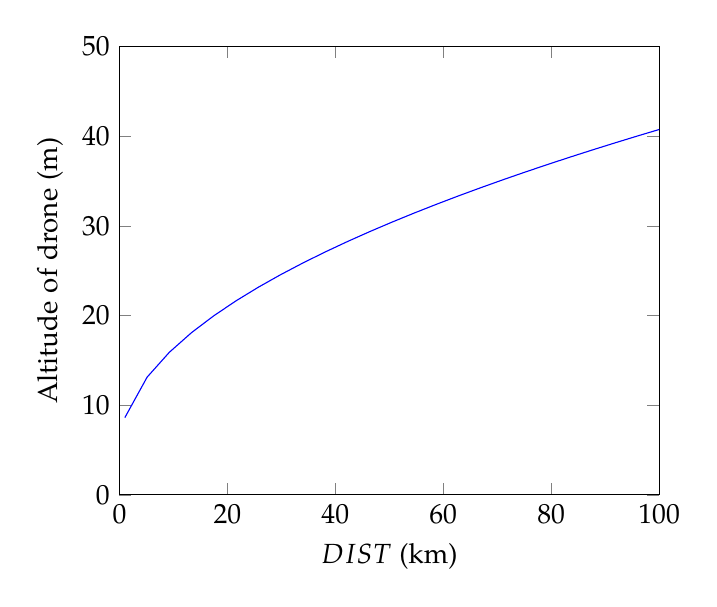
\begin{tikzpicture}
 \begin{axis}[ 
	xmin=0,
	xmax=100,
	ymin=0,
	ymax=50,
    domain = 1:100,
    xlabel=$DIST$ (km),
    ylabel={Altitude of drone (m)}
  ] 
    \addplot+[mark=none,unbounded coords=jump] {3.57 * (sqrt(2) + sqrt(x))}; 
  \end{axis}
\end{tikzpicture}
\caption{Graph for distance as a function of drone altitude}
\label{fig_maxdist}
\end{figure}
\section{Power vs. signal strength}

Signal strength created by an increase in power follows exactly the same formula, is a constant for any power ratio (regardless of distance covered), and is:

$$dB = 10*log \frac{P1}{P2}$$

\section{433 vs 900 Mhz}
Given the same amount of power in both systems, the 433mhz will give more range, 

%\pagebreak

\bibliographystyle{plain}
%https://en.wikipedia.org/wiki/Line-of-sight_propagation
\bibliography{bibfile}
%----------------------------------------------------------------------------------------
%\end{multicols}
\end{document}
